%Path explosion problem is still the main obsticale against scaling up symbolic execution to industrial sized projects.
%%
%One interesting resolution to the problem is \emph{Veritesting}, which represents regions of code as disjunctive formals over paths.
%%
%Unlike the C compiler that inlines functions in programs, Integrating veritesting with Java bytecode presents unique challenges: notably, incorporating non-local control jumps caused by runtime polymorphism, exceptions, native calls, and dynamic 3 class loading.
%%
%In this paper we present our robust implementation of Java based veritesting tool that supports dynamic dispatch and
\section{Introduction}
\vaibhav{needs rewriting, assigned to anyone who can find the time to write it}

Symbolic execution is a popular analysis technique that performs non-standard execution of a program: data operations generate formulas over inputs, and the branch constrains along an execution path are combined into a predicate.
%
Originally developed in the 1970s~\cite{King1976,Clarke1976}, symbolic execution is a convenient building block for program analysis, since arbitrary query predicates can be combined with the logical program representation, and solutions to these constraints are program inputs illustrating the queried behavior.
%
Some of the many application of symbolic execution include
test generation~\cite{dart,cute}, equivalence checking~\cite{ramos,adaptorsynth}, vulnerability finding~\cite{driller,angr}, and protocol correctness checking~\cite{transport}.
%
Symbolic execution tools are available for many languages, including
CREST~\cite{BurnimS2008} for C source code, KLEE~\cite{CadarDE2008}
for C/C++ via LLVM, JDart~\cite{jdart2016} and Symbolic
PathFinder~\cite{spf} for Java, and S2E~\cite{ChipounovKC2012},
FuzzBALL~\cite{BabicMMS2011}, and angr~\cite{angr} for binary code.
%
 \mike{More here...explain the `ecosystem' - tools for different languages: KLEE, FuzzBall, Java Symbolic Pathfinder, ...}

Although symbolic analysis is a very popular technique, scalability is a substantial challenge for symbolic execution.
%
Dynamic state merging~\cite{kuznetsov} provides one way to
alleviate scalability challenges by opportunistically merging dynamic
symbolic executors, which can be performed on paths~\mike{Add std. cite} or on environments~\mike{FM paper from 2014 on Javascript?}.  
Other techniques include CEGAR/subsumption~\mike{Add references from ASE 2017 paper: More Effective Interpolations in Software Model Checking}.
 
%
Veritesting~\cite{veritesting} is a different recently proposed technique that can dramatically improve the performance of symbolic execution.  Rather than explicitly merge paths or check subsumption relationships, Veritesting simply encodes a local region of a program containing branches as a disjunctive region for symbolic analysis.  If any path within the region meets an exit point, then the disjunctive formula is satisfiable.  This often allows many paths to be collapsed into a single path involving the region.  
%
In previous work~\cite{veritesting}, bounded static code regions have been shown to find more bugs, and achieve more node and path coverage, when implemented at the X86 binary level for compiled C programs.
%
This provides motivation for investigating integration of introducing static regions with symbolic execution at the Java bytecode level.

\lstinputlisting[caption={An example to loop through a symbolic array with three execution paths through the loop body},
label={lst:v_ex}]{code_samples/VeritestingPerf.java}



%Symbolic Pathfinder~(SPF)~\cite{spf} is a tool that performs symbolic execution of Java bytecode.
%
%SPF is tightly integrated with Java PathFinder~(JPF)~\cite{jpf} and uses JPF extensions to replace concrete execution with symbolic execution.
%
We present an example demonstrating the potential benefit of integrating static code regions with SPF in Listing~\ref{lst:v_ex}.
%
The example checks if positive or negative integers occur more frequently in the
list~\textit{x}, and it contains a bug if \textit{x} contains an
equal number of positive and negative integers.
%
The three-way branch on lines 5, 6 causes the total number of execution
paths required to cover the \textit{for} loop to be $3^{\textit{len}}$.
%
However, this three-way branch can be combined into a multi-path region
and represented as a disjunctive predicate.
We present such predicates in SMT2 notation in
Listing~\ref{lst:v_ex_smt2} assuming \textit{x} to contain two symbolic
integers named \textit{x0} and \textit{x1}~(\textit{len} equals 2).
%
The updates to \textit{sum} in the two loop iterations are captured by
\textit{sum0} and \textit{sum1}.
%
Using such predicates to represent the three-way branch on lines 5, 6 of
Listing~\ref{lst:v_ex} allows us to have only one execution path through
the loop body.
%
Figure~\ref{fig:v_ex_plot} shows a comparison of the number of execution
paths explored to find the bug on line 11 of Listing~\ref{lst:v_ex}.
%
The exponential speed-up from our predicates, representing a multi-path
region, allows us to find
the bug using just three test cases.

Unfortunately, as originally proposed, Veritesting would be unable to create a static region for this loop because it involves non-local control jumps (the calls to the \texttt{get} methods).  This is not an impediment for compiled C code, as the C compiler will usually automatically inline the code for short methods such as \texttt{get}.  However, Java has an {\em open world} assumption, and most methods are {\em dynamically dispatched}, meaning that the code to be run is not certain until resolved at runtime, so the compiler is unable to perform these optimizations.

In Java, programs often consist of many small methods that are dynamically dispatched, leading to poor performance for n\"aive implementations of bounded static regions.  Thus, to be successful, we must be able to inject the static regions associated with the calls into the dispatching region.  We call such regions {\em higher order} as they require a region as an argument and can return a region that may need to be further interpreted.
Given support for such regions, we can make analysis of programs such as~\ref{lst:v_ex} trivial for large loop depths.  In our experiments, we demonstrate 100x speedups on several models (in general, the more paths contained within a program, the larger the speedup) over the unmodified Java SPF tool using this approach.
 
%
\lstinputlisting[caption={SMT2 representation of multi-path execution in
Listing ~\ref{lst:v_ex} using \textit{len} = 2}, label={lst:v_ex_smt2}, language=lisp]{code_samples/ex.smt2.snippet}
%
\begin{figure}[]
\caption{Comparing number of execution paths from Listing~\ref{lst:v_ex} using vanilla SPF and SPF with static unrolling}
\label{fig:v_ex_plot}
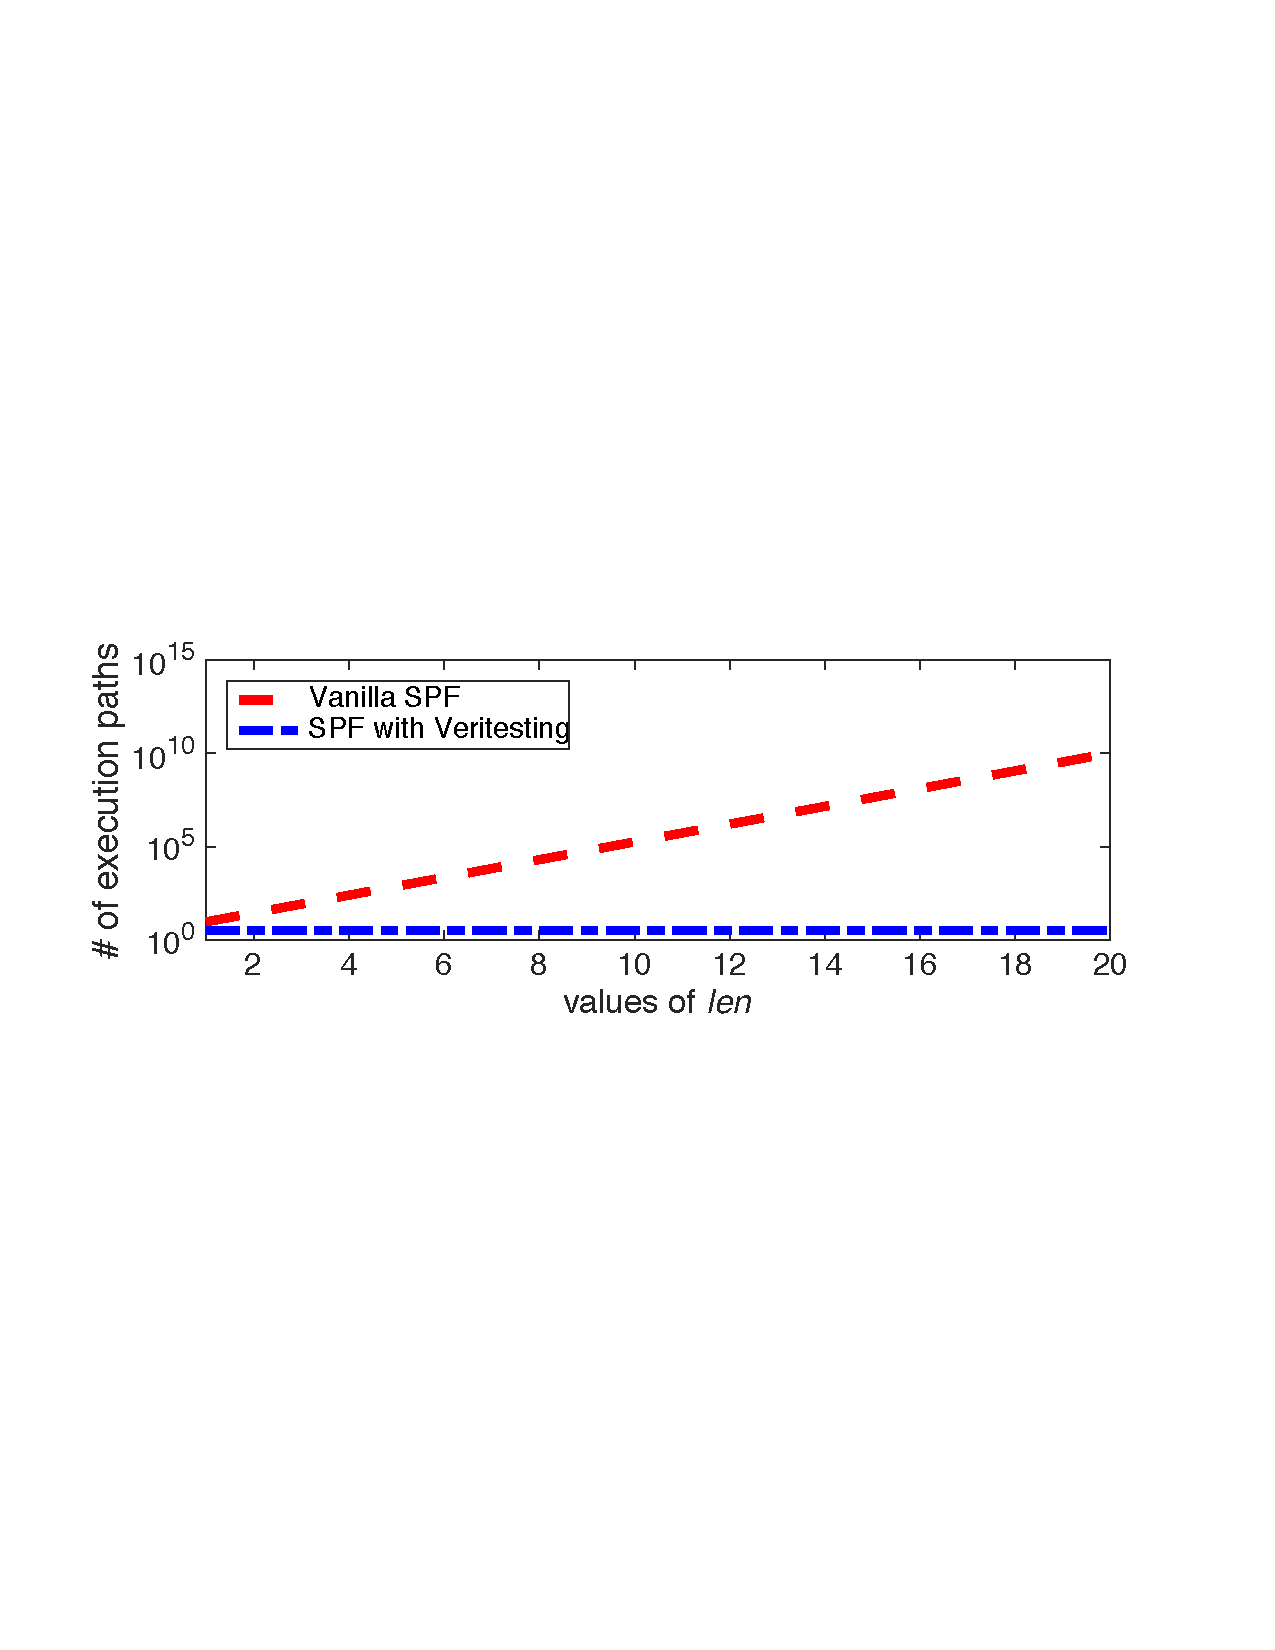
\includegraphics[width=\columnwidth]{figures/veritesting_example_semilogy}
\end{figure}
%
\subsection{Motivating Example}
\vaibhav{assigned to Vaibhav}
%\begin{figure}[h]
% \centering
% \begin{subfigure}[b]{0.48\textwidth}
%  \centering
%  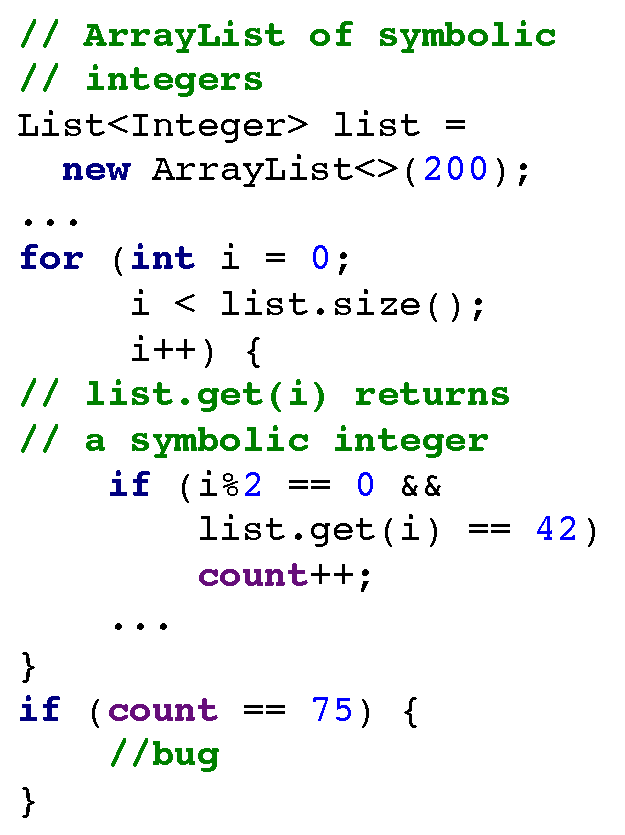
\includegraphics[width=\textwidth]{figures/example.pdf}
%  \caption{asdf}
% \end{subfigure}\hfill%
% %
% \begin{subfigure}[b]{0.48\textwidth}
%  \centering
%  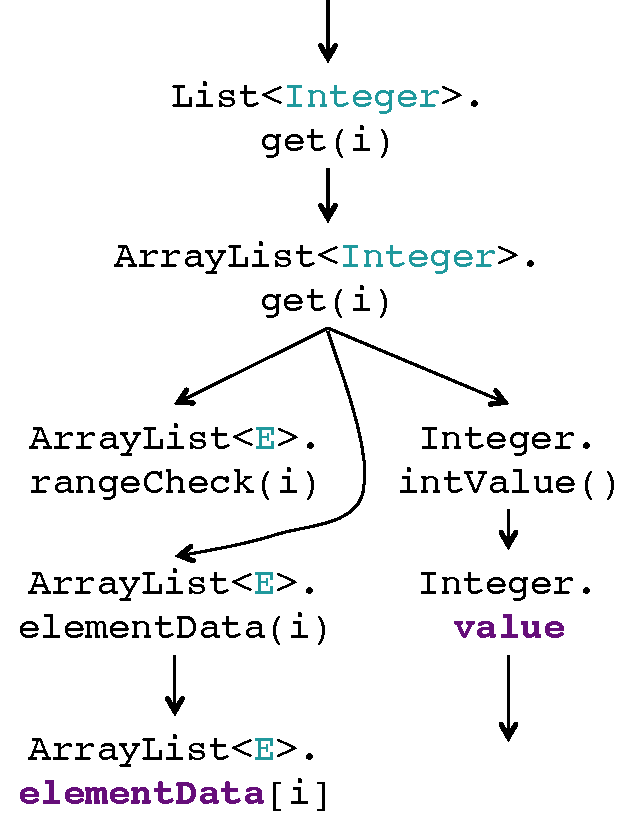
\includegraphics[width=\textwidth]{figures/example-flow.pdf}
%  \caption{}
% \end{subfigure}%
% \caption{Some caption}
% \label{fig:mot-example}
%\end{figure}
\begin{figure}
    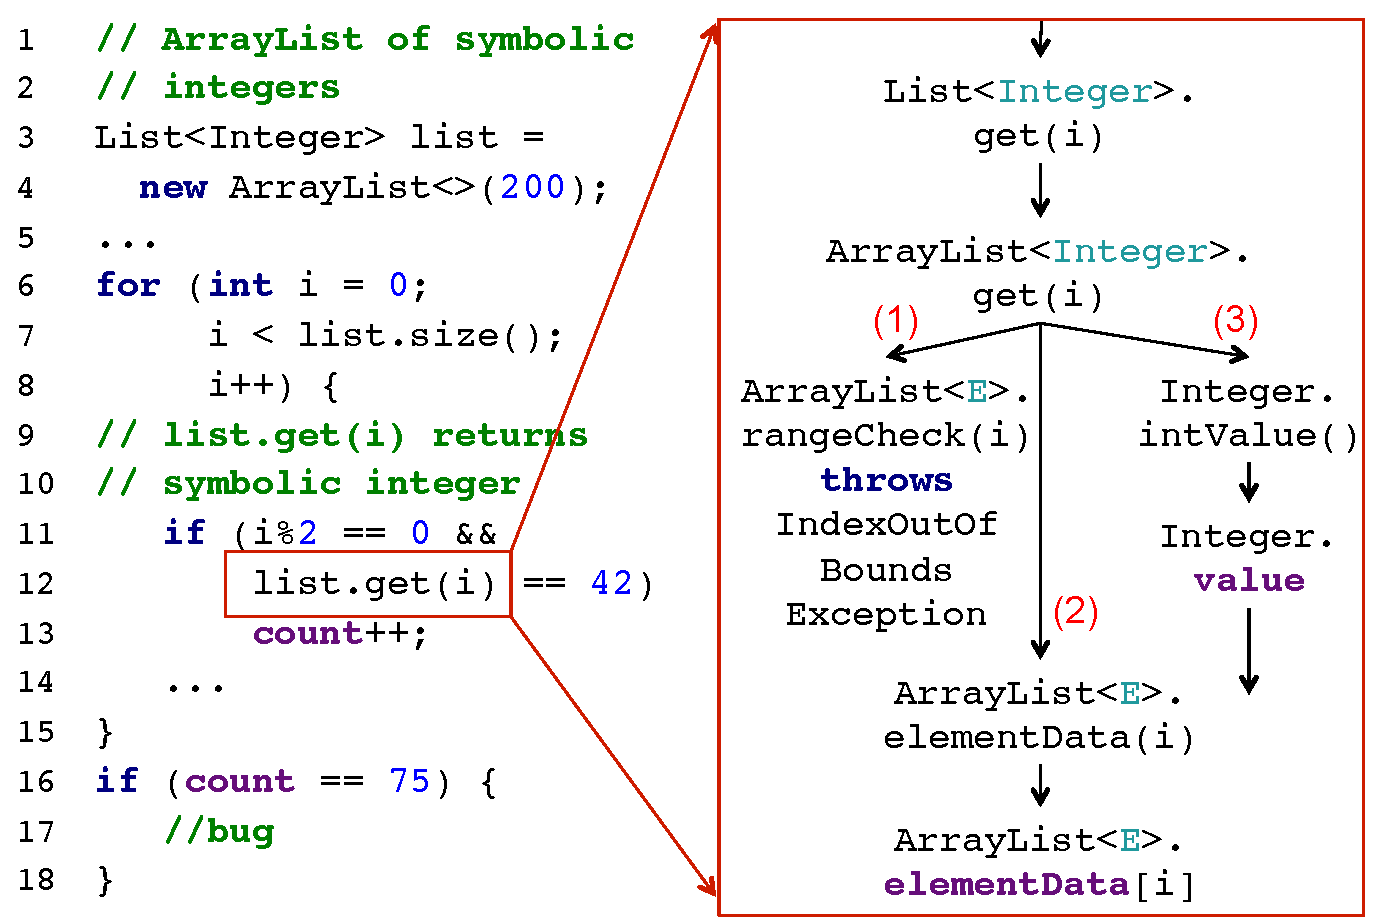
\includegraphics[width=\textwidth]{figures/example-combined.pdf}
    \caption{Some caption}
    \label{fig:mot-example}
\end{figure}
Consider the example shown in Figure \ref{fig:mot-example}.